\usetikzlibrary{shapes.geometric};


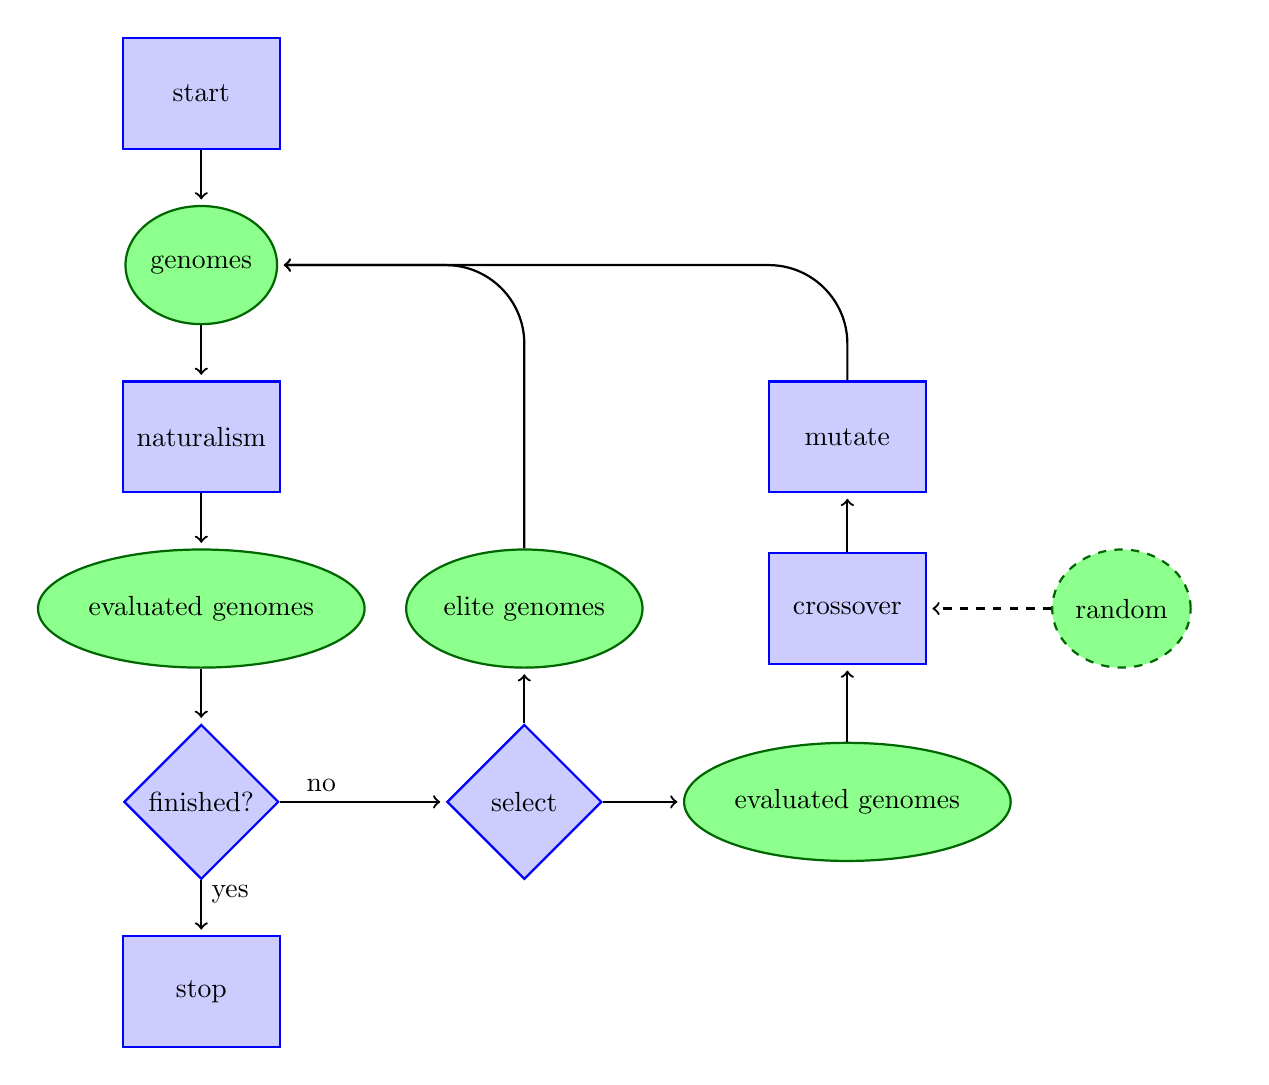
\begin{tikzpicture}
	[auto,
		decision/.style	={diamond
									, draw=blue
									, thick, fill=blue!20
									, text width=4.5em
									, align=flush center
									, inner sep=1pt
									},
		block/.style		={rectangle
% 									, rounded corners
									, draw=blue
									, thick, fill=blue!20
									, text width=5em
									, align=center
									, minimum height=4em
									},
		line/.style		 	={draw
									, thick
									, ->
									,shorten >=2pt
									},
		cloud/.style		={ellipse
									, rounded corners
									, draw=green!40!black
									, thick
									, fill=green!45!white
									, minimum height=1.5cm
									, inner sep=1pt
									}
	]
\matrix [column sep=5mm,row sep=7mm]
	{
		% row 1

			\node [block] (start) {start}; & 
		\\
		% row 2
			\node [cloud] (genomes 1)					{genomes}; &
			&
		 \\
		% row 3
			\node [block] (naturalism)						{naturalism}; &
			&
			\node [block] (mutate)							{mutate}; &
		\\
		% row 4
			\node [cloud] (evaluated genomes 1)	{evaluated genomes}; & 
			\node [cloud] (elite genomes)				{elite genomes}; & 
			\node [block] (crossover)						{crossover}; &
			\node [cloud, dashed] (random)							{random}; &
		\\
		% row 5
			\node [decision] (finished)								{finished?}; & 
			\node [decision] (select)								{select}; & 
			\node [cloud] (evaluated genomes 2)	{evaluated genomes}; &


		\\
		% row 6

			\node [block] (stop)								{stop}; &
		\\
	};
\begin{scope}[every path/.style=line, rounded corners=1cm]

	\path					(start)					-- (genomes 1);
	\path					(mutate) 				|- (genomes 1);
	\path					(genomes 1) 		-- (naturalism);
	\path					(elite genomes) 	|- (genomes 1);
	\path					(crossover) 			-- (mutate);
	\path	[dashed]	(random)-- (crossover);
	\path					(naturalism)			-- (evaluated genomes 1);
	\path					(select)				-- (elite genomes);
	\path					(evaluated genomes 2)-- (crossover);
	\path					(finished) 				--node [near start] {yes}(stop);
	\path					(finished) 				--node [near start] {no}(select);
	\path					(select)				-- (evaluated genomes 2);
	\path					(evaluated genomes 1) --(finished);
\end{scope}
\end{tikzpicture}

